\documentclass[a4paper, 12pt]{article}
\usepackage{geometry}
\geometry{a4paper,
total={170mm,257mm},left=2cm,right=2cm,
top=2cm,bottom=2cm}

\usepackage{mathtext}
\usepackage{amsmath}
\usepackage[T2A]{fontenc}
\usepackage[utf8]{inputenc}
\usepackage[english,russian]{babel}
\usepackage{graphicx, float}
\usepackage{tabularx, colortbl}
\usepackage{caption}
\captionsetup{labelsep=period}

\newcommand{\parag}[1]{\paragraph*{#1:}}
\DeclareSymbolFont{T2Aletters}{T2A}{cmr}{m}{it}
\newcounter{Points}
\setcounter{Points}{1}
\newcommand{\point}{\arabic{Points}. \addtocounter{Points}{1}}
\newcolumntype{C}{>{\equation*ing\arraybackslash}X}

\author{Калинин Даниил, Б01-110}
\date{\today}
\title{Лабораторная работа 4.3.2A Дифракция света на ультразвуковой волне в жидкости}

\begin{document}
\maketitle
\parindent=0cm

\parag {Цель работы}
изучение дифракции света на синусоидальной 
акустической решётке и наблюдение фазовой решётки методом тёмного поля.

\parag {В работе используются}
оптическая скамья, осветитель,
светофильтры, конденсор, щель, 2 длиннофокусных объектива,
кювета с водой, кварцевый излучаетль с микрометрическим винтом,
генератор УЗ-частоты, частотомер, линза, отсчётное устройство,
микроскоп.

\parag {Теоритическая справка} ~\\
\par При прохождении ультразвуковой (УЗ) волны через жидкость в ней 
возникают периодические оптические неоднородности, обусловленные 
разницей значений коэффициента преломления в областях сжатия и 
разрежения. Эти периодические неоднородности играют роль своеобразной 
дифракционной решётки для проходящего сквозь жидкость света.\\
\par При небольших амплитудах звуковой волны показатель преломления 
жидкости n меняется по закону

\begin{equation*}
    n = n_0(1 + m cos(\Omega x))
\end{equation*}

где $\Omega$ - волновое число для УЗ-волны ($\Omega = \frac{2\pi}{\Lambda}$), 
$\Lambda$ - длина УЗ-волны, m - глубина модуляции показателя преломления, определяемая
интенсивностью ультразвуковой волны ($m \ll 1$)

\par Пусть фаза световых колебаний на передней поверхности жидкости равна
нулю. Тогда на задней поверхности (т.е. в плоскости $z = 0$) она равна

\begin{equation*}
    \varphi = knL = \varphi_0(1 + m cos(\Omega x))
\end{equation*}

\par Можно сформулировать качественный критерий, при выполнении которого
можно считать акустическую решётку чисто фазовой, т.е. рассматривать её 
как тонкий фазовый экран. Для нашей задачи условие тонкого транспаранта 
можно записать в виде

\begin{equation*}
    m \ll \frac{\Lambda}{L}\sqrt{\frac{\lambda}{L}}
\end{equation*}

\par Проведённое рассмотрение дифракции на фазовой решётке справедливо 
только в случае слабой фазовой модуляции. В общем случае после прохождения
через кювету световое поле представляет совокупность не трёх, а 
большого числа плоских волн, распространяющихся под углами, 
определяемыми условием

\begin{equation*}
    \Lambda sin\Theta_m = m\lambda~~(m = 0, \pm1, \pm2,...)
\end{equation*}

\par Каждая из этих волн соответствует одному из максимумов в 
дифракционной картине Фраунгофера.
\par Определяя на опыте положение дифракционных максимумов различного 
порядка, можно по формуле (4) найти длину $\Lambda$ УЗ-волны и вычислить
скорость $v$ распространения ультразвуковых волн в жидкости, если 
известна частота $\nu$ колебаний кварцевого излучателя

\begin{equation*}
    v = \Lambda \nu
\end{equation*}

\parag {Экспериментальная установка}~\\
Схема установки представлена на рисунке \ref{pic:setup}.

\begin{figure}[h]
    \centering
    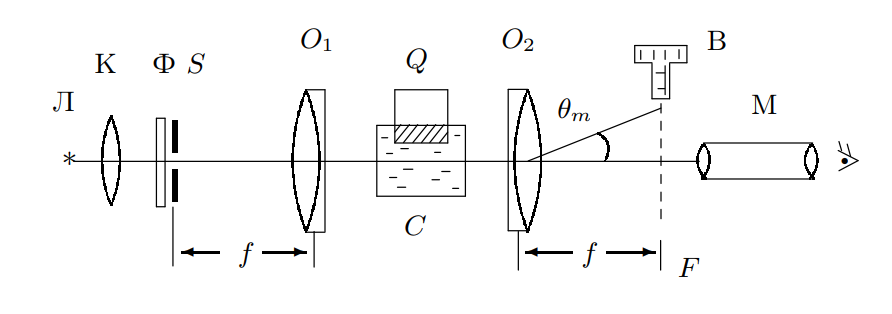
\includegraphics[scale = 0.6]{setup.png}
    \caption{Схема экспериментальной установки}
    \label{pic:setup}
\end{figure}

\parag {Ход работы} ~\\
\point Собераем схему согласно описанию.

\point Настраиваем микроском, далее выставляем ширину щели в 25мкм.

\point Подбирая частоту генератора, получаем дифракционную картину
в объективе микроскопа. $\nu = 1.037 \pm 0.001$ МГц

\point Крутя лимб находим расстояние между соседними наиболее чёткими
дифракционными картинами. $d = 760 \pm 10$ мкм, т.е. длина
УЗ-волны порядка $1.520 \pm 0.02$ мм

\point Рассчитываем скорость звука в воде $1580 \pm 20 \frac{м}{с}$

\point Измеряем координаты дифракционных максимумов для разных частот. Результаты занесем в таблицы \ref{tabl:data_1}, \ref{tabl:data_2}, \ref{tabl:data_3} соответственно.

\begin{table}[H]
    \centering
    \begin{tabular}{|c|c|c|c|c|c|c|c|c|c|c|}
        \hline
        \multicolumn{8}{|c|}{$\nu = 1.037$ МГц}                      \\ \hline
        m             & 1   & 2   & 3   & 4   & 5   & 6   & 7        \\ \hline
        $x_m$, дел    & 57  & 88  & 120 & 150 & 181 & 214 & 244      \\ \hline
    \end{tabular}

    \caption{Координаты дифракционных максимумов на частоте $\nu = 1.037$ МГц}
    \label{tabl:data_1}
\end{table}

\begin{table}[H]
    \centering
    \begin{tabular}{|c|c|c|c|c|c|c|c|c|c|c|}
        \hline
        \multicolumn{8}{|c|}{$\nu = 1.109$ МГц}                      \\ \hline
        m             & 1   & 2   & 3   & 4   & 5   & 6   & 7        \\ \hline
        $x_m$, дел    & 60  & 88  & 121 & 153 & 190 & 226 & 258      \\ \hline
    \end{tabular}

    \caption{Координаты дифракционных максимумов на частоте $\nu = 1.109$ МГц}
    \label{tabl:data_2}
\end{table}

\begin{table}[H]
    \centering
    \begin{tabular}{|c|c|c|c|c|c|c|c|c|c|c|}
        \hline
        \multicolumn{6}{|c|}{$\nu = 1.209$ МГц}          \\ \hline
        m             & 1   & 2   & 3   & 4   & 5        \\ \hline
        $x$, дел      & 85  & 118 & 157 & 195 & 233      \\ \hline
    \end{tabular}

    \caption{Координаты дифракционных максимумов на частоте $\nu = 1.209$ МГц}
    \label{tabl:data_3}
\end{table}

\point На основе каждой таблицы построим графики зависимости $x(m)$, изобразим их на рисунках \ref{fig:graph_1}, \ref{fig:graph_2}, \ref{fig:graph_3} соответственно.

\begin{figure}[H]
    \centering
    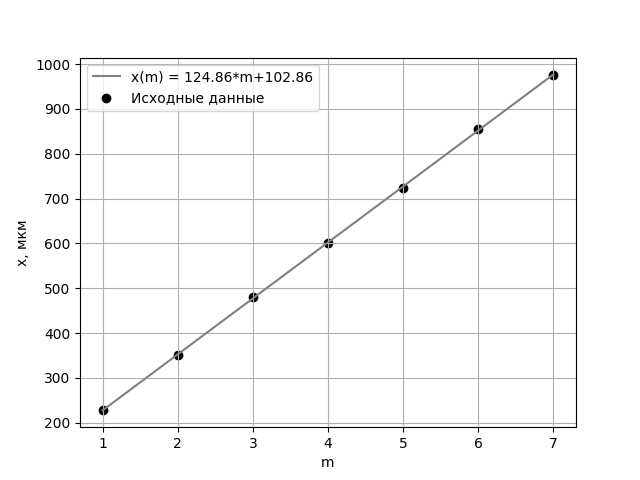
\includegraphics[width=0.6\linewidth]{graph1.png}
    \caption{x(m) при $\nu = 1.037$ МГц}
    \label{fig:graph_1}
\end{figure}

Определим длину волны по углу наклона графика:
\begin{center}
    $\frac{l_m}{m} = \frac{\Delta x_m}{\Delta m} = 125$ мкм,
    $\Lambda = \frac{\lambda f}{l_m/m} = 1590$ мкм,
    $\varepsilon_{\Lambda} = 5.8$\%
\end{center}

\begin{figure}[H]
    \centering
    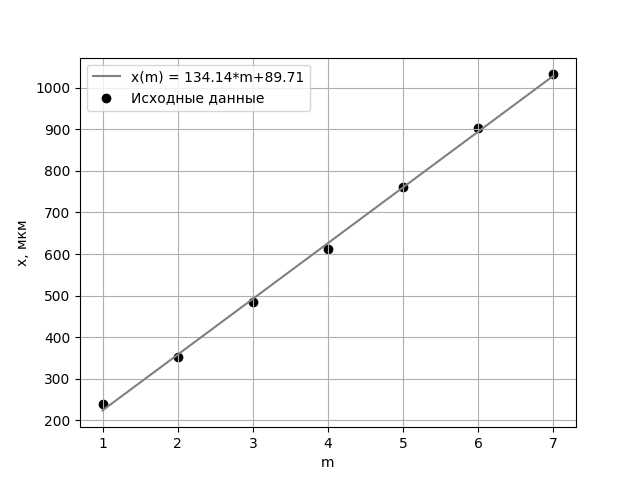
\includegraphics[width=0.6\linewidth]{graph2.png}
    \caption{x(m) при $\nu = 1.109$ МГц}
    \label{fig:graph_2}
\end{figure}

Определим длину волны по углу наклона графика:
\begin{center}
    $\frac{l_m}{m} = \frac{\Delta x_m}{\Delta m} = 134$ мкм,
    $\Lambda = \frac{\lambda f}{l_m/m} = 1430$ мкм,
    $\varepsilon_{\Lambda} = 5.7$\%
\end{center}

\begin{figure}[H]
    \centering
    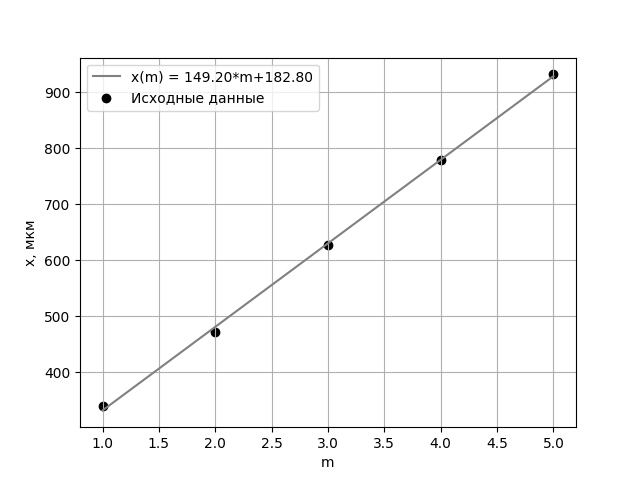
\includegraphics[width=0.6\linewidth]{graph3.png}
    \caption{x(m) при $\nu = 1.209$ МГц}
    \label{fig:graph_3}
\end{figure}

Определим длину волны по углу наклона графика:
\begin{center}
    $\frac{l_m}{m} = \frac{\Delta x_m}{\Delta m} = 149$ мкм,
    $\Lambda = \frac{\lambda f}{l_m/m} = 1290$ мкм,
    $\varepsilon_{\Lambda} = 5.5$\%
\end{center}

\point Отмечаем координаты на шкале микроскопа, совпадающие с соседними 
линиями сетки (0.20 мм и 1.02 мм)

\point Проведем измерения методом темного поля и расчитаем скорость звка для каждой частоты. Результат занесем в таблицу \ref{tabl:data_dark_field}.

\begin{table}[H]
    \centering
    \begin{tabular}{|c|c|c|c|c|c|}
        \hline
        $\nu$, МГц & 1-я полоса & последняя полоса & кол-во светлых полос & $\Lambda$, мкм & $v$, $\dfrac{м}{с}$    \\ \hline
        1.068      & 0.4        & 3.64             & 6                    & 1317           & 1407                   \\ \hline
        1.096      & 0.22       & 3.42             & 6                    & 1300           & 1425                   \\ \hline
        1.127      & 0.2        & 3.84             & 7                    & 1268           & 1429                   \\ \hline
        1.156      & 0.06       & 3.66             & 7                    & 1254           & 1450                   \\ \hline
        1.186      & 0.04       & 3.48             & 7                    & 1199           & 1422                   \\ \hline
        1.216      & 0          & 3.38             & 7                    & 1178           & 1432                   \\ \hline
    \end{tabular}
    \caption{Результаты измерения скорости звука}
    \label{tabl:data_dark_field}
\end{table}

\parag {Заключение} ~\\
В ходе работы было изучено явление дифракции света на стоячей УЗ-волне
в воде. Была измерена скорость звука в воде 2-мя способами: по дифракционной
картине и методом тёмного поля, оба способа привели к рещультату, совпадающему
с табличным с учётом погрешности, но метод тёмного поля оказался более точным.
\end{document}
